\chapter{Foundations}
\label{foundations}
In this chapter we describe the foundations and concepts necessary to understand the work proposed in this thesis. First we explain about Software Reuse, its state-of-art, its benefits, challenges, code-search engines, component retrieval techniques, and ranking components. Then we talk about Continuous Integration, its benefits, challenges, and successful CI practices. We finalize this chapter by describing Microservices and its characteristics.
\section{Software Reuse}
\label{chap:sw-reuse}
Douglas McIlroy \cite{McIlroy1968} envisaged in the 1960s a software system composed of already existent components. Where you basically put different components, that already exist, together in order to form the system is being built. One can depict this vision using LEGO where the system is a group of pieces put together, and each of those pieces is a component.

Although the IT industry has tried for many years to improve the speed and reduce costs of software development by reusing components, the McIlroy's vision is still the exception rather than the rule.

Despite the fact that it is possible to find several definitions of software reuse in the literature, most of them are similar to the definition proposed by Krueger \cite{Krueger1992}:

\textit{"Software reuse is the process of creating software systems from existing software rather than building software systems from scratch"}

Since we already have a formal definition of software reuse, the next question would be: What can be reused?. To this regard, the work of \citeauthor{Frakes1996} defined a list (Table \ref{reusable-list}) of potentially reusable software artifacts, where you can find architectures, source code, requirements, etc.

\begin{table}[]
\centering
\label{reusable-list}
	\begin{tabular}{|l|l|}
		\hline
		1. architecture						 & 6. estimates (templates) \\ \hline
		2. source code  						 & 7. human interfaces      \\ \hline
		3. data                               & 8. plans                 \\ \hline
		4. designs                            & 9. requirements          \\ \hline
		5. documentation                      & 10. test cases           \\ \hline
	\end{tabular}
	\caption{Potentially reusable aspects of software projects according to \cite{Frakes1996}.}
\end{table}

However, reuse traditionally means the reuse of code fragments and components \cite{Mili2002}. When we talk about components, we mean any cohesive and compact unit of software functionality with a well defined interface \cite{Hummel2008}. Therefore a component can be a simple classes or even a web-service or Enterprise Beans.

Software reuse emerges as a solution for the so called software development crisis \cite{Kim1992}. Organizations face several problems in software development including increased costs, delayed schedules, unsatisfied requirements, and software professional shortage. Therefore, by reusing software components projects can reduce time-to-market, lower development costs, and increase software quality \cite{Frakes2005}.

\subsection{Benefits of Software Reuse}
Software reuse has not failed to attract the attention of industry due to its alleged benefits. In the industry the need of reduction of redundancies, as well as costs reduction and quality improvements is perceived. Moreover, the vision of fostering innovation and market penetration due to shorter production cycles promised obvious strategic business advantages \cite{Bauer2016}. Research literature has reported benefits from successful adoption of software reuse:

\begin{itemize}
\item Lower cost and faster development
\item Higher quality
\item Standardized architecture
\item Risk reduction
\end{itemize}

Unfortunately the adoption of suitable reuse strategy is pretty challenging as it takes place in a multifaceted environment and, thus, incorporates aspects ranging from technical to organizational at different level of abstractions \cite{Bauer2016}.

\subsection{Challenges of Software Reuse}
\label{sec:sw-challenges}
Although software reuse brings many benefits, as we stated before, it has failed to take off. Find the right third-party software component to be reused based on a well-defined specification is one of the most challenging approaches due to the fact that it requires a clear-cut matching of the potential reuse candidate and the given specification. Although there are several search tools available, most of them are still text-based and it neither reflect nor support the need to match the reuse candidates with the syntactic and semantic characteristics of a specification \cite{Hummel2013}. \citeauthor{Hummel2013}, based on software retrieval literature, identified fours problems for implementing a sustainable reuse repository.

\begin{itemize}
\item Repository problem \cite{Seacord1999}: This reuse repository should create and maintain a big enough software collection to provide promise search.
\item Representation problem \cite{Pole1994}: The repository should represent and index its content in a way that makes it easily accessible.
\item Usability problem \cite{Garcia2006}: The repository should permit characterizing a desired component with reasonable effort and precision.
\item Retrieval problem \cite{Prieto-Diaz1987}: The repository should execute the queries with high precision to retrieve the desired component.
\end{itemize}

Although the two first challenges have been address in the last years, the last two have not been addressed completely. By the rise of open-source movement and the improvements in the Internet connectivity, software developers have got access to vast swathes of free software, thus the problem of sources of components is not problem any more. Furthermore, with the advances in database and text search technologies code-search engines have made the creation of \textit{Internet-scale} software repositories wherefore this repository problem can be regarded as solved \cite{Hummel2013}. For the second problem, clever ranking approaches such as the ranking proposed by \cite{Inoue2005} which ranks those components higher in the result list of a search that are more often used than others amongst the indexed files. Moreover, the idea of parsing source code in order to extract objects and their method introduced by Koders.com, where techniques that addressed the representation problem. However, the last two problems remain still in the focus of interest in the research community.

Beside the technical problems described above, organizational challenges and human factors have been identified as potential inhibitors to a successful implementation of reuse practices \cite{Morisio2002}. Business strategy, management commitment, and company culture are organizational factors that might affect software reuse \cite{Standish1984}. Moreover, technical problems are strongly related to human factors, such as cognitive efforts, program understanding, and motivation. In the work of \cite{Bauer2016} the following organizational obstacles were identified in the literature:

\begin{itemize}
\item Organization structure: Factors like competition, overlapping or unclear responsibilities, priority conflicts, and lack of coordination of reuse activities jeopardize the successful of reuse implementation. 
\item Inertia: Some organizations usually assess their managers and developers based on the success of their isolated projects, which incentives local optimization which impact reuse in a company-wide scale. 
\item Knowledge: If an organization plans to implement reuse practices, it needs clear position organization-wide and research into current methods and techniques for reuse.
\item Management: As implementing reuse practices require changes in governance strategies, it causes additional overhead that tends to be underestimated in the initial planning, which put at risk successful of reuse.
\item Economic: Implementation of reusability requires investment and long-term support from management to resolve restrictive resource constraints.
\item Disincentives: The quality of the reusable component candidates is one of the strongest disincentives. Moreover the criteria applied to measure developers and managers have an impact on their motivation to take part into reuse.
\end{itemize}

\subsection{Code-search engines}
Code-search engines are the heart of the new generations of reuse support tools. For example, Code Conjurer \cite{Hummel2008} uses Merobase component search engine, CodeGenie relies on Sourcerer \cite{Lemos2007} or ParseWeb that works over Google Code Search \footnote{Shutdown January, 15 2012 \cite{Horowitz2011}} \cite{Thummalapenta2007}. Next we will describe some code search engines that are still online the time of this work.

\begin{itemize}
\item searchcode\footnote{https://searchcode.com/ (accessed: 13.01.2017)} searchcode is a free source code search engine. Code snippets and open source (free software) repositories are indexed and searchable. Most information is presented in such a way that you shouldn't need to click through, but can if required.
\item NerdyData\footnote{https://nerdydata.com (accessed: 13.01.2017)} It is a search engine for source code. It supports HTML, Javascript and CSS. With this search engine you can retrieve the web pages which are using a specific file. For example if you look up for \textit{font-awesome.min.css} it will retrieve the sites that are using this file.
\item Spars-J\footnote{http://sel.ist.osaka-u.ac.jp/SPARS/ (accessed: 13.01.2017)} It is a keyword and name matching code search engine on open source XML, Java and JSPs based on component rank and keyword rank algorithm.
\item ComponentSource\footnote{https://www.componentsource.com/ (accessed: 13.01.2017)} It is a keyword-matching of component descriptions in a marketplace. Here you can find components for different platforms and technologies.
\item Satsy: It is a source code search engine that implemented semantic search using input/output queries on mutil-path programs with ranking. Based on survey to 30 participants, it retrieved more relevant results than Merobase \cite{Stolee2016}.
\item Merobase\footnote{http://www.merobase.com/ - Official project deprecated, we use a local implementation} Merobase is a component search engine that uses Lucene \footnote{Apache LuceneTM is a high-performance, full-featured text search engine library written entirely in Java. It is a technology suitable for nearly any application that requires full-text search, especially cross-platform \cite{lucene}.} to index programming language units from various open source repositories (such as Sourceforge, Google Code, or the Apache projects) and the open Web. Merobase, when crawling the code, its analysis software identifies the basic abstraction implemented by a module and stores it in a language agnostic description format. This description includes the abstraction's name, methods names, parameter signatures, among others.
\end{itemize}

Although Google or Yahoo! are not specialized code search engines, they are able to return more precise results than code search engines\cite{Hummel2007}.

\subsubsection{Merobase}
\label{subsec:merobase}

Merobase contains special parsers for each supported programming languages (currently it supports Java, C++, and C\#, also it supports WSDL files, binary Java classes from JARs and .NET binaries), which extracts syntactical information, stores it in the index and search for it later. Moreover, it contains a special parser for JUnit which is able to extract the interface of the class under test from test cases.

Every time a user make a request to Merobase, the parsers described above are invoked and try to extract as much syntactic information from the query as possible. If none of the parsers recognizes parsable code in the query, it executes a simple keyword search. Based on parsed syntactic information, Merobase supports retrieval by class and operation names, signature matching and by matching the full interface of classes described before.

When a JUnit test case is submitted, a test-driven search is triggered. In this case, Merobase automatically tries to compile, adapt and test the highest ranked candidates. If a candidate is relying on additional classes, the algorithm uses dependency information to locate them as well. It is important to point out that the actual compilation and testing are not carried out on the search server itself, but on dedicated virtual machines within sandboxes. This is due to the fact that this ensures that the executed code does not have the possibility to do anything harmful to the user's system or bring the whole testing-environment down \cite{Hummel2013}.

The current implementation of Merobase, which will we used in our prototype, has been enhanced in several way since the implementation described above \cite{Kessel2016}. Many new metrics are measured on the software components, both statically and dynamically, when the test cases executed on them. Also, the semantic retrieval of components has been improved by adding a better parser for Java components which supports the creation of entire class hierarchies. With this, information about the components' class hierarchies can be retrieved and stored.

On the other hand, the current implementation is populated with software components extracted from Maven projects mainly extracted from the Maven Central Repository\footnote{https://repo1.maven.org/maven2/ (accessed: 15.01.2017)}. 

\subsection{Component retrieval techniques}
As we stated in \ref{sec:sw-challenges}, several problems of software reuse have been already addressed. Now one of the big problems is how to choose the so-called best component. In this section we will talk about the different component retrieval techniques proposed in the literature. Then we will explain further what test-driven component retrieval means.

\cite{Mili1998} divided the component retrieval techniques in six independent groups:

\begin{itemize}
\item Information retrieval methods: It is basically the methods of information retrieval used for retrieving candidates by applying textual analysis to software assets. This group has high recall and medium precision.
\item Descriptive methods: These methods add additional textual description of assets such as keyword or facet definition, to the textual analysis. These are high precision and high recall.
\item Operational semantic methods: These methods use sampling of assets to retrieve candidates. They have very high precision and high recall.
\item Denotational semantic methods: These methods use signature methods for retrieving candidates. The have very high precision and high recall.
\item Structural methods: These methods deal with the structure of the components to retrieve candidates. This group has very high precision and recall.
\item Topological methods: This is an approach to minimize the distance between query and reusable candidates. It is difficult to estimate or define recall and precision for these methods \cite{Mili1998}.
\end{itemize}

Although \cite{Mili1998} proposed six groups, the last one relies on a \textit{measurable} retrieval techniques so it can be considered as an approach for ranking the candidate components of a query \cite{Hummel2007}.

In the work \cite{Hummel2007} several retrieval techniques were compared. They compared signature matching, text-based, name-based and interface-driven. These techniques were tested using Merobase search engine. The result they obtained was that the best technique is interface-driven in terms of precision.

Another technique that was presented in \cite{Hummel2004}, is test-driven search. This technique ruses test cases as a vehicle to retrieve the component candidates that fit better the requirements of the user. It promises to improve the precision of the searches in comparison with other techniques explained before. Below we will explain with further details how this techniques works. 

\subsubsection{Test-driven search}
Simple techniques for component retrieval such as keyword-driven search or signature-driven search may lead to a tons of candidates from which just a small group might be interesting for the user, in spite of the results fulfill the search criteria. This is due to the fact that not all of them fulfill the functional properties of the desire artifact. Here is were test-driven search comes to light. 

Test-driven reuse approach was first introduced in \cite{Hummel2004}. It is a technique that emerges as a solution to the problem of retrieving so many irrelevant component candidates due to large amount of component in a repository. Specifically this technique deals with the usability and retrieval problems we explained before. It relies on test cases written by user (step a), then it extracts the different interfaces defined in the test case (step b), then it makes the search of reuse candidate (step c). Then it run the tests and \textit{cleans} the result set of candidates that do not pass the tests (step d and e). Finally it shows the cleaned result set to the user (step f). This is the test-driven reuse cycle which can be seen in the figure \ref{fig:test-driven-cycle}.

\begin{figure}[ht]
	\centering
    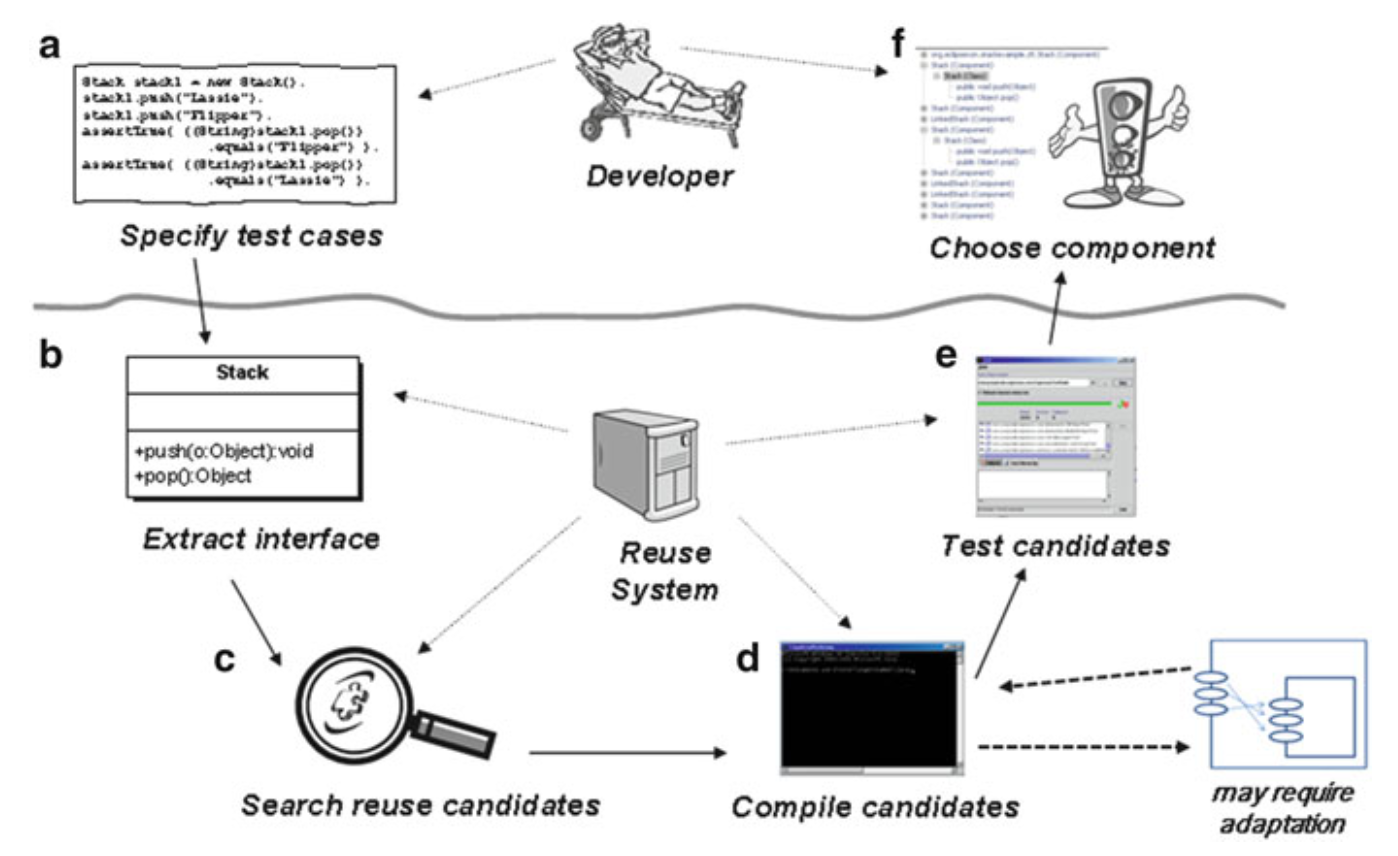
\includegraphics[width=\textwidth]{grafiken/test-driven-cycle}
    \caption{The test-driven reuse \textit{cycle} extracted from \cite{Hummel2013}}
    \label{fig:test-driven-cycle}
\end{figure}

An implementation of this \textit{cycle} is Code Conjurer which can be found in \cite{Hummel2008} and\cite{Hummel2013}. This implementation is an Eclipse plugin that delivers proactively reuse recomendations by silently monitoring the user's work and triggering searches automatically whenever this seems reasonable. This tool supports interface-base searches and test-driven searches. For the latter, the tool has a background agent that monitors the required interface of the JUnit test case (also called, \textit{class under test} (CUT)) written by the developer. When a change in the CUT happens, Code Conjurer sends the JUnit test to Merobase where the interfaces are extracted and used to search for results. Then the candidates retrieved are tested against the test provided and the candidates that do not pass the tests are removed. Finally the candidates are shown to the user in Eclipse.

Another tools that uses test-driven search are S6 \cite{Reiss2009} and CodeGenie \cite{Lemos2007}.

This approach for searching candidates is very promising because of popularity of Agile practices and specifically of Test-Driven development (TDD)\cite{Beck2003}. In TDD developers writes the tests of the desired component before writing a single line of its implementation. Therefore, the chances of finding a component that can be reused instead of writing it from scratch is pretty high. We will explain TDD with further details is Section \ref{sec:tdd}.

In spite of the fact that this search method retrieves more relevant resources, it needs improvement in order to be applicable for the daily work of a developer. The amount of time taken from submitting the test case till receive the results is sometimes excessive, this is due to the fact that each candidate needs to be compiled and validated against the test case. Although this problem can be overcome by increasing the resources, it brings extra costs. 

\subsection{Ranking components}
Retrieving components is not enough. The problem that emerge with retrieving components using code-search engines is when several candidates meet the functional requirements. Which of them is the best?. Normally engines sort the results by keyword or text matching thus the first component in the list is not necessary better than the last one. This is because factors such as ... are not being considered for ranking the components.

\subsubsection{SOCORA}
The ranking component approach presented in \cite{Kessel2016} works as follow. First, it establishes a partial ordering of candidates using non-dominated sets determined by non-dominated sorting without assuming any preferences of the user. Depending on the priorities assigned to each selected criterion, it then subrank each non-dominated set in a recursive way until all unique priorities and their corresponding subcriteria are applied to the current level of non-dominated sets, eventually resulting in nested subrankings. Note that in each step, when (new)non-dominated sets are determined by non-dominated sorting, the ranks of sets may change according to their partial ordering. In general, partial subranking are deliberately supported since the user is not required to assign specific priorities to all his/her selected criteria. The priorities are defined by simple integer values (highest value represent more priority than a lower value) with a default priority assignment of 1 for each selected criterion. If the user wants to assign a higher or lower priority to a selected criterion, he/she may increase or decrease the priority by 1 or even a larger number. Both unique and equal priority values may be assigned to selected criteria to establish either a partial or strict ordering. For each priority value, all corresponding criteria are selected to subrank each non-dominated set of non-distinguishable candidates. This process starts with the highest priority value and continues in descending order until the smallest priority value is reached \cite{Kessel2016}. The figure \ref{fig:socora-ex} is a schematic illustration of how the component ranking works.

\begin{figure}[ht]
	\centering
    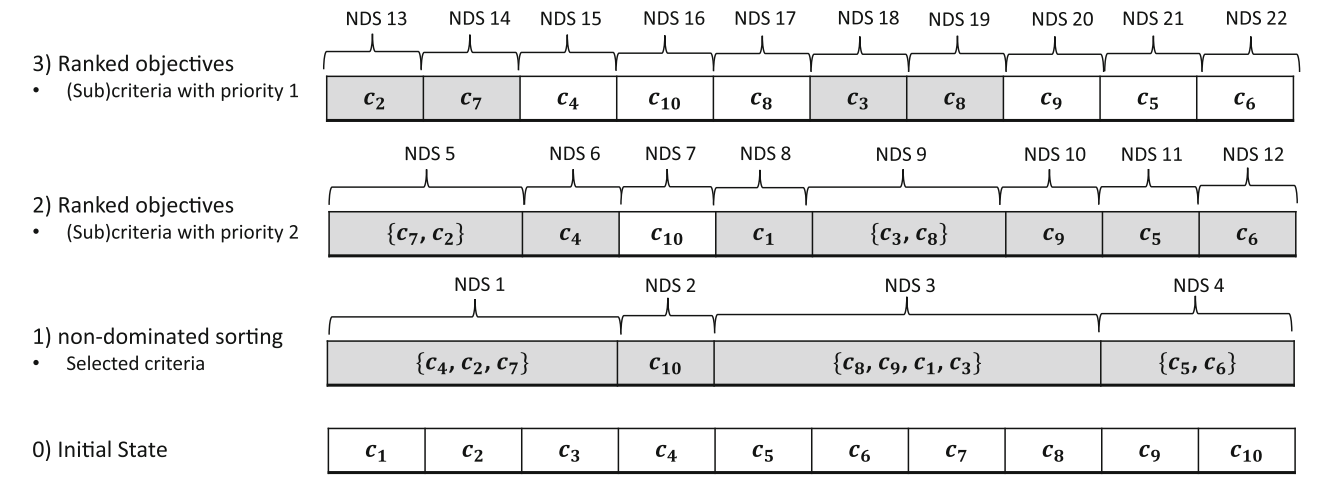
\includegraphics[width=\textwidth]{grafiken/socoraExample}
    \caption{Schematic illustration of SOCORA ranking approach \cite{Kessel2016}}
    \label{fig:socora-ex}
\end{figure}

\paragraph{Merobase integration}

The prototype of the ranking component approach is integrated with the component search engine Merobase to retrieve the candidates. The figure \ref{fig:socora-merobase} shows how SOCORA\footnote{SOCORA prototype http://socora.merobase.com (accessed: 13.01.2017)} is integrated with Merobase. 

\begin{figure}[ht]
	\centering
    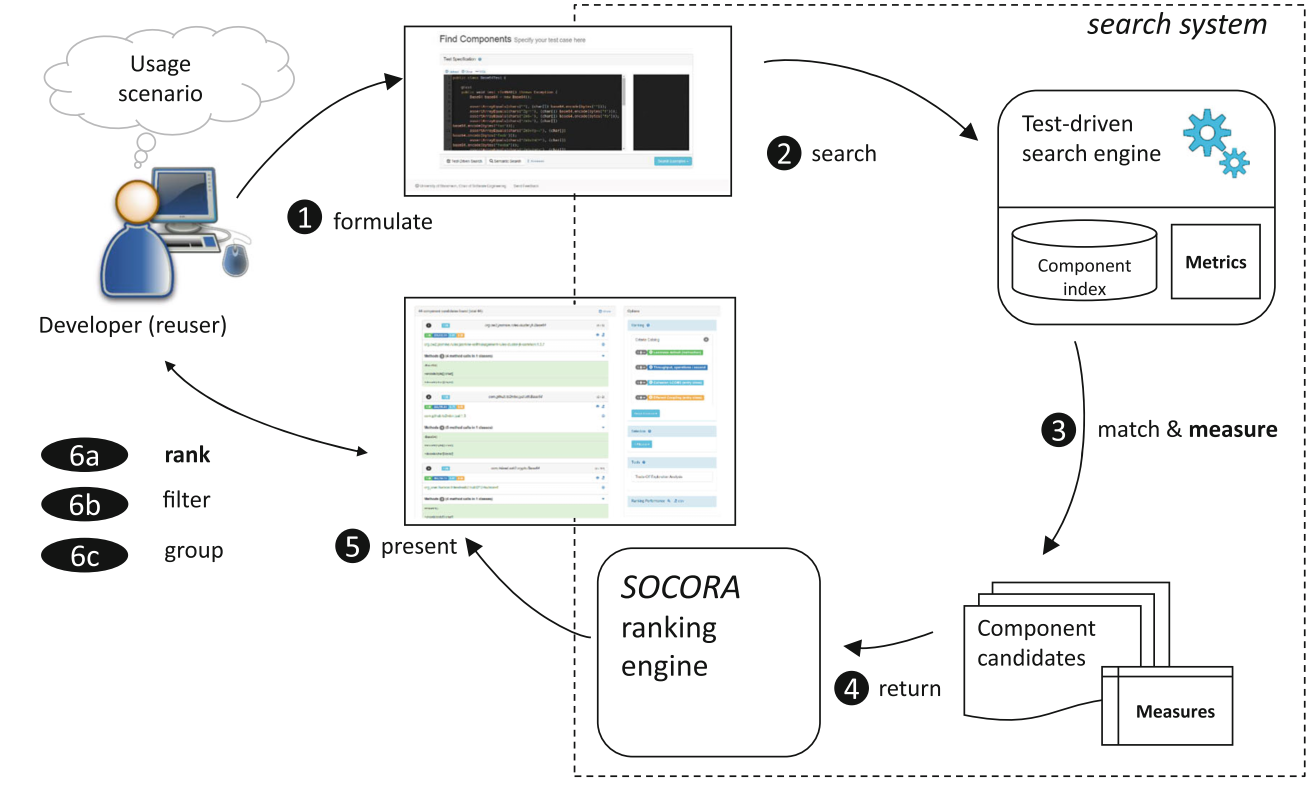
\includegraphics[width=\textwidth]{grafiken/socora-merobase}
    \caption{SOCORA and Merobase integration (extracted from \cite{Kessel2016})}
    \label{fig:socora-merobase}
\end{figure}

In the first step the user's functional requirements are described as a JUnit test specification using a HTML5 web-based GUI. Here the user can specify a set of non-functional \textit{quality} criteria that he/she thinks to be important for his/her needs, also he/she optionally can provide relative priorities to partially order them. In the second step, the interface signatures in the JUnit test are extracted and a text-based search is performed in order to find suitable components. In the step 3, the result set of component from the second step are filtered by applying the JUnit test in turn, and those that do not match the filtering criteria are removed. Also, during the compilation and execution of the test, the metric selected by the user are evaluated. In the step 4, the information from the last step is used by the ranking algorithm to order the remaining components in the result set. In the step 5 the remaining components in the result set are displayed to the user. In the last step, the user can further analyze the component candidates by exploring the effects of different partial ordering (step 6a), explore different criteria (step 6b), and can group them in different way to shrink the result set (step 6c).